\input sys/inputs.tex
\usepackage[czech]{babel}

\begin{document}

\bigheading{Lyžování}

% \info{task_name}{infile}{outfile}{points}{timelimit}{memlimit}
% leave this values, if you are not interested
\info{skiing}{stdin}{stdout}{100}{1000 ms}{1 GB}

Po neúspěšném pokusu dostat se na IOI se Kleofáš rozhodl stát se mistrem ve slalomu na lyžích.
Zítra je pro Kleofáše nadmíru důležitý den: bude se konat jeho první lyžařský závod!

Během soutěžního sjezdu se bude muset Kleofáš dostat z počátečního bodu do cílového
a přitom projet $n$ brankami. Jelikož jde samozřejmě o to být co nejrychlejší,
chce Kleofáš použít nejkratší možnou trasu.

\heading{Úloha}

Pro náš popis sjezdovky je důležitý počáteční bod $S$, koncový bod $F$ a pozice $n$ 
branek. Každou branku si lze představit jako úsečku rovnoběžnou s $x$-ovou (vodorovnou) osou. Žádné dvě branky
nemají stejné $y$-ové souřadnice (výšku). Počáteční bod leží nad každou brankou, tj. jeho $y$-ová souřadnice je vyšší
než $y$-ová souřadnice libovolné branky; a podobně koncový bod leží pod každou brankou.

Vaším úkolem je najít nejkratší lomenou čáru, která začíná v $S$, končí v $F$ a prochází všemi brankami,
a to \textbf{seshora dolů}. Přitom \textbf{stačí}, aby lomená čára procházela krajním bodem branky.

\heading{Vstup}

První řádek vstupu obsahuje celé číslo $n$ ($0 \leq n \leq 10^6$) -- počet branek.
na druhém řádku jsou celá čísla $x_S, y_S, x_F, y_F$: souřadnice počátku $S = (x_S, y_S)$,
resp. konce $F = (x_F, y_F)$.

Následuje $n$ řádků, z nichž $i$-tý obsahuje celá čísla ${x_1}_i, {x_2}_i, {y}_i$, která říkají, že $i$-tá branka
je úsečka s krajními body $({x_1}_i, y_i)$ a $({x_2}_i, y_i)$. Vždy platí ${x_1}_i < {x_2}_i$.

Všechny souřadnice jsou mezi $-10^9$ a $10^9$ včetně. Branky jsou seřazeny shora dolů, tj. platí
$y_S > y_1 > y_2 > \dots > y_n > y_F$.

\heading{Výstup}

Lze dokázat, že vždy existuje právě jedna nejkratší lomená čára vyhovující zadání a že souřadnice všech jejích vrcholů jsou celočíselné.
Vypište vrcholy této lomené čáry, a to bez zbytečných vnitřních vrcholů (tj. v každém vypsaném vnitřním vrcholu lomená čára musí změnit směr).

\begin{center}
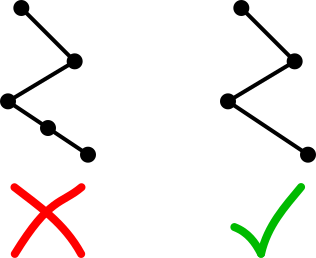
\includegraphics[width=5cm]{img/skiing1}
\end{center}

Na první řádek výstupu vypište celé číslo $k$ -- počet vrcholů hledané lomené čáry.
Dále vypište $k$ řádků a na $i$-tém z nich dvě mezerou oddělená celá čísla $x_i, y_i$ -- souřadnice $i$-tého vrcholu lomené čáry.
Vrcholy musí být uvedeny v pořadí od počátku ke konci, tj. musí platit
$x_1 = x_S, y_1 = y_S, x_k = x_F, y_k = y_F$ a $y_1 > y_2 > \dots > y_k$.

\heading{Podproblémy}

\begin{center}
\begin{tabular}{|l|l|l|l|}
\hline
podproblém & body & nejvyšší $n$                 \\ \hline
1       & 20     & 200                                          \\ \hline
2       & 30     & 2000                                         \\ \hline
3       & 50     & 1000000                                        \\ \hline
\end{tabular}
\end{center}

\heading{Příklady}


\sampleIN
4
5 10 6 0
0 4 7
7 10 6
5 8 4
2 5 1
\sampleOUT
5
5 10
4 7
7 6
5 1
6 0
\sampleCOMMENT
Situace vypadá následovně:
\sampleEND
\center{
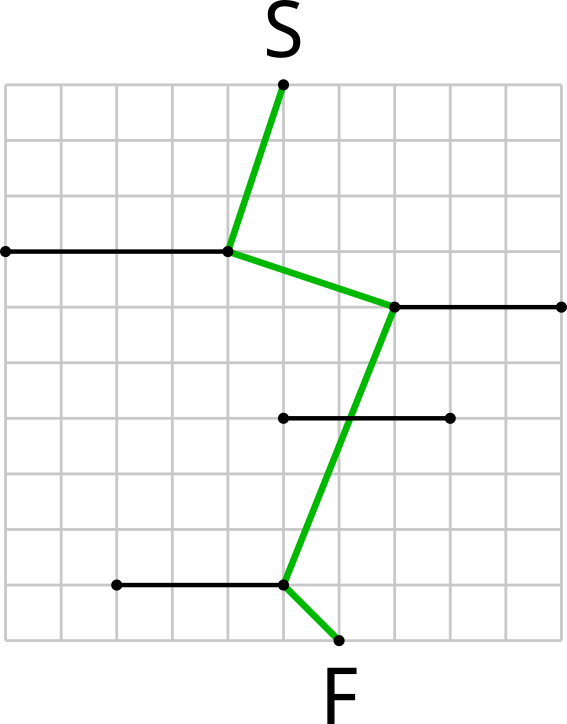
\includegraphics[width=6cm]{img/skiing2}
}

\end{document}
